\section{Serial Logging}

The state-of-the-art algorithm for serial logging is ARIES. In ARIES, each log record consists of one modified data tuple and the name of the transaction that modifies the tuple. It is assigned a log sequence number in ascending order. The log records are first pushed to volatile storage and then flushed to nonvolatile storage after the transaction is committed. Two data structures are maintained: the Dirty Page Table and the Transaction Table. The DPT keeps track of all the changes made to the database that have not been flushed to the disk, and the transaction table records all the transactions that are currently running in the system. During the recovery process, the system first recovers and updates the dirty page table and the transaction table, then recovers the system to the state immediately before the crash, and finally undoes all the transactions that have not been committed.\par
%Explain ARIES%
In our implementation of ARIES, we simplified the algorithm such that each transaction is logged together and corresponds to one unique LSN. Each transaction goes to log only after it is committed. This makes the dirty page table unnecessary, and we do not need to undo during the recovery process because only the committed transactions are reflected in stable storage. \par

A key insight of logging is that we need to maintain the dependency between different transactions. For example, in the following case on the left, Transaction 1 writes to tuple A and Transaction 2 read tuple A. If Transaction 2 is logged before the system crash whereas Transaction 1 is not, during the recovery processs, Transaction 2 will be reading the wrong data. Hence, Transaction 2 must go to log after Transaction 1 has already been logged. 
\begin{figure}[!h]
\caption{Transaction dependencies: RAW and WAW}
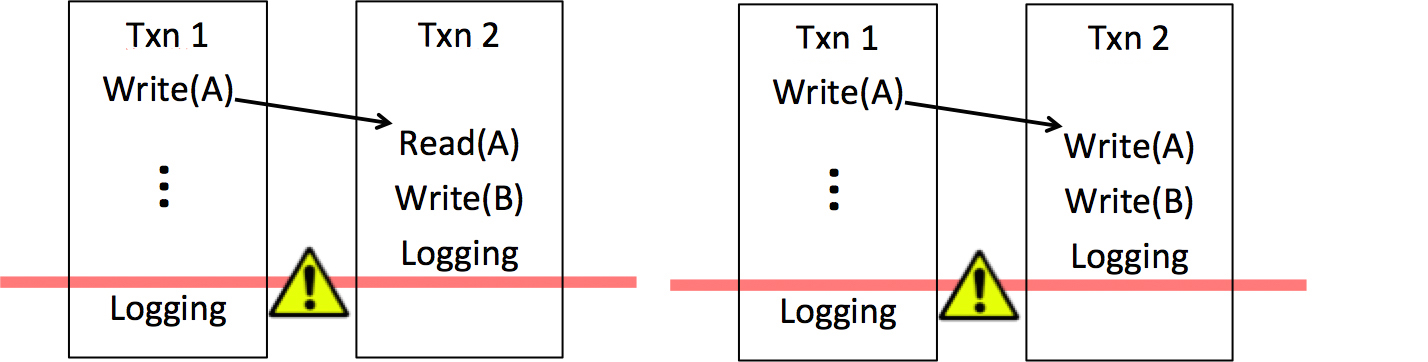
\includegraphics[width=\textwidth]{DepExample.jpeg}
\end{figure}\\
The above type of transaction dependency is called read-after-write (RAW). In general, there are four types of transaction dependencies:
\begin{itemize}
\item Read-after-read dependency (RAR)
\item Read-after-write dependency (RAW)
\item Write-after-read dependency (WAR)
\item Write-after-write dependency (WAW)
\end{itemize}
RAR is equivalent to no dependency since no changes are made to the database. RAW has been discussed above, and WAW has to be maintained because in the example on the right, during recovery, transaction 2 will overwrite a phantom value of tuple A that cannot be tracked down in the system. Therefore, the reading transaction (2) should go to log after the writing transaction (1).\par
Since it is necessary to maintain different types of dependencies between pairs of transactions, the serial logging algorithm assumes that all dependencies have to be maintained and therefore logs the transactions one by one in sequential order. Our paper argues that this viewpoint is too conservative, and we propose the parallel algorithm, where we track down the types of transaction dependency to minimize the number of dependencies that we need to maintain. This involves a discussion of the WAR dependency. For more details, please refer to the parallel logging section. \par

\textcolor{red}{[TODO] Justin's optimization of serial logging algorithm}

